\documentclass[11pt]{article}
\usepackage[a4paper,margin=2.3cm]{geometry}
\usepackage[T1]{fontenc}
\usepackage[utf8]{inputenc}
\usepackage{lmodern}
\usepackage{amsmath,amssymb}
\usepackage{booktabs}
\usepackage{xcolor}
\usepackage{tikz}
\usetikzlibrary{positioning,arrows.meta,fit}
\usepackage[colorlinks=true,linkcolor=blue!50!black,citecolor=blue!50!black,urlcolor=blue!50!black]{hyperref}

\newcommand{\measured}{\textnormal{\textsc{[measured]}}}
\newcommand{\proposed}{\textnormal{\textsc{[proposed]}}}
\newcommand{\projected}{\textnormal{\textsc{[projected]}}}

\title{Toward a Citizen AI on 1{,}000 Consumer GPUs:\\
Data-Efficient JEPA Language Models for HiveMind's OpenTrainer and OpenRouter\\
\large Proposal paper}
\author{Xavier Callens\\ \small Project HiveMind}
\date{15 November 2026}

\begin{document}
\maketitle

\begin{abstract}
HiveMind aims at a \emph{citizen AI}: language models trained and served by volunteers' consumer GPUs and coordinated
by two open services, OpenTrainer (training) and OpenRouter (serving). We propose an evolution of HiveMind around
JEPA-style training objectives, which promise more learning per token at little or no extra compute, the two resources
a volunteer network lacks.

The paper keeps three layers apart:
\begin{itemize}
\item \measured: what we observed on our own hardware;
\item \proposed: what we design and have implemented as opt-in, CPU-tested code;
\item \projected: estimates for a 1{,}000-node network, every input stated as an assumption.
\end{itemize}

\textbf{Measured.} LLM-JEPA gave no gain on a 658M volunteer-trained base model with LoRA rank 64. It degraded general
loss by $0.90$ nat through a collapse of its cosine term. Stop-gradient, centering and InfoNCE removed the damage, but
did not produce a gain. The model's largest weakness is its data mix (code $+3.84$ nat).

\textbf{Proposed.} We make Semantic Tube Prediction (STP) the first candidate: it needs no paired views and no extra
forward pass. We provide a document-aware, replay-deterministic implementation; a new OpenTrainer task type carrying a
signed objective specification; and three experimental OpenRouter model types.

\textbf{Projected.} A per-node budget for 1{,}000 consumer GPUs, and the coordination bottlenecks that must be removed
first, starting from today's fleet of one physical GPU.

All new experiments are pre-registered and gated; no production path changes without a passed gate.
\end{abstract}

\section{Introduction}
A citizen AI is one whose training and serving are carried by the public's own machines rather than by a single
operator. HiveMind builds the coordination for this: OpenTrainer dispatches signed training work to volunteers (through
an HTTPS relay, AMCP over Kafka, or BOINC night workunits), and OpenRouter serves OpenAI-compatible requests from
volunteer producers.

The honest starting point \measured:
\begin{itemize}
\item the serving fleet is \textbf{three producer accounts on one physical GPU}, and 12 of 14 catalog models have a
single producer (\texttt{docs/GEN6\_VERIFIED\_SWARM\_DESIGN\_2026-11-01.md});
\item the BOINC server runs with \textbf{one volunteer host} (\texttt{docs/BOINC\_PRODUCTION\_SERVER.md});
\item the training cell is an RTX 2070 (8\,GB) and a Tesla T4 (16\,GB).
\end{itemize}
A thousand consumer GPUs is three orders of magnitude away.

Two things make the gap worth attacking with the training objective itself.
\begin{itemize}
\item Volunteer compute is scarce and heterogeneous: 8--12\,GB cards that can fine-tune adapters of 0.6--3B models, not
pretrain them.
\item Curated data is scarce too: our volunteer-trained model is far behind a same-size industrial model on code and
mathematics (Section~\ref{sec:measured}).
\end{itemize}
An objective that extracts more from each token at no extra compute would help on both counts. LLM-JEPA
\cite{huang2025llmjepa} and Semantic Tube Prediction \cite{huang2026stp} are such candidates, at least by their
authors' claims.

\section{Background}
\paragraph{LLM-JEPA.} Next-token loss plus $\lambda\,(1-\cos)$ between the last-token hidden states of two \emph{paired
views} of the same content (e.g.\ a description and its regex) \cite{huang2025llmjepa}. Its cost is about $2\times$,
because of an extra forward pass. The paper reports $+11.4$ points at LoRA rank 64 on NL-RX-SYNTH for an
instruction-tuned 1B model.

\paragraph{Semantic Tube Prediction (STP).} The authors' follow-up \cite{huang2026stp} posits that token sequences trace
near-geodesics in hidden space, and adds
\begin{equation}
\mathcal{L}_{\text{STP}} = 1-\cos\big(h_t-h_r,\ h_r-h_s\big),\qquad s<r<t \text{ random},
\end{equation}
on last-layer states of the \emph{same} forward pass. It needs no paired views, and its overhead is ``negligible''. The
paper claims the same accuracy as regular fine-tuning with $16\times$ less data on NL-RX-SYNTH. It evaluates
fine-tuning of Instruct models only; pretraining is not tested. The released code
(\texttt{galilai-group/llm-jepa}) also contains a different ``random span'' variant that the paper does not describe;
we treat the two as distinct.

\paragraph{Distributed training.} OpenTrainer rounds follow DiLoCo \cite{douillard2023diloco}: local inner steps, then
an outer Nesterov step on the averaged deltas. Robust aggregation (Multi-Krum \cite{blanchard2017krum}) and a held-out
loss ratchet exist in the CrowdGPT bridge. BOINC \cite{anderson2004boinc} carries night workunits, whose results are
checked by deterministic replay. Adapters are QLoRA \cite{dettmers2023qlora}.

\section{What we measured \measured}
\label{sec:measured}
All on a shared Tesla T4 with Crowd-v1 (658M trunk parameters), under a guard that keeps 4.3\,GB of VRAM free for live
inference. The details are in a companion report \cite{callens2026crowd}.

\begin{table}[h]
\centering\small
\caption{Measured results that motivate this proposal (companion report \cite{callens2026crowd}).}
\label{tab:measured}
\begin{tabular}{p{4.1cm}p{10.2cm}}
\toprule
Experiment & Result\\
\midrule
Held-out evaluation & The project's loss check ignored the model's engram table ($+0.35$ nat). Fixed; the signed
receipt now binds it.\\
LLM-JEPA, pre-registered & LoRA r64, $\lambda{=}1$, 3 seeds: $16.90\pm1.06\%$ vs $17.07\pm0.93\%$ exact match; general
loss $+0.90$ nat; cosine term collapses to $\le5\times10^{-4}$.\\
Compute-matched screen & 10 hypotheses, 5 tested: stop-gradient, centering and InfoNCE remove the collapse; none beats
SFT at equal compute (best ties it).\\
Per-domain gap to Qwen3-0.6B & code $+3.84$, math $+2.44$, encyclopedic $+1.80$, science $+1.50$, educational web
$+1.04$, own data $+0.36$ nat.\\
\bottomrule
\end{tabular}
\end{table}

\paragraph{Two lessons.}
\begin{enumerate}
\item A JEPA term that compares raw final states can be satisfied by a shortcut: every state drifts toward one shared
direction. That shortcut harmed general language modeling. STP compares \emph{displacements}, in which a shared offset
cancels; we expect it to resist that shortcut, but this is our reasoning, not a measurement.
\item The largest lever for the volunteer model is data, not the objective. Any objective must be evaluated next to a
data-mix change.
\end{enumerate}

\section{Proposed evolution \proposed}
\begin{figure}[t]
\centering
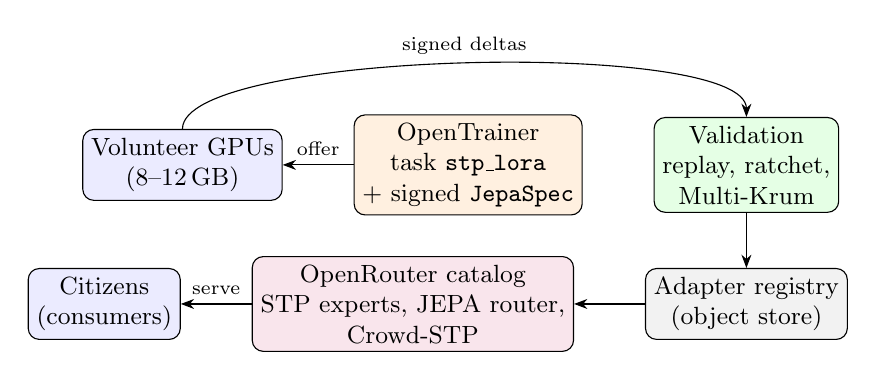
\begin{tikzpicture}[node distance=7mm and 9mm, box/.style={draw, rounded corners, align=center, font=\small,
  minimum height=9mm, inner sep=3pt}, >={Stealth}]
\node[box, fill=blue!8] (vol) {Volunteer GPUs\\ (8--12\,GB)};
\node[box, fill=orange!12, right=of vol] (ot) {OpenTrainer\\ task \texttt{stp\_lora}\\ + signed \texttt{JepaSpec}};
\node[box, fill=green!10, right=of ot] (val) {Validation\\ replay, ratchet,\\ Multi-Krum};
\node[box, fill=gray!10, below=of val] (reg) {Adapter registry\\ (object store)};
\node[box, fill=purple!10, left=of reg] (or) {OpenRouter catalog\\ STP experts, JEPA router,\\ Crowd-STP};
\node[box, fill=blue!8, left=of or] (cons) {Citizens\\ (consumers)};
\draw[->] (ot) -- node[above, font=\scriptsize]{offer} (vol);
\draw[->] (vol.north) .. controls +(0,1.0) and +(0,1.0) .. node[above, font=\scriptsize]{signed deltas} (val.north);
\draw[->] (val) -- (reg);
\draw[->] (reg) -- (or);
\draw[->] (or) -- node[above, font=\scriptsize]{serve} (cons);
\end{tikzpicture}
\caption{Proposed flow. Every arrow except the objective specification exists today. The new parts are the
\texttt{stp\_lora} task, the signed \texttt{JepaSpec}, the adapter registry for large deltas, and the experimental
catalog entries.}
\label{fig:arch}
\end{figure}

\subsection{An opt-in JEPA library}
\texttt{src/hivemind/jepa} is implemented with 9 CPU tests:
\begin{itemize}
\item a versioned, validated objective spec whose SHA-256 is bound into signed workunits; clients refuse unknown
versions;
\item the paper's STP loss, \emph{document-aware}: triples never cross an end-of-document token in packed streams, which
the paper never faced;
\item \emph{deterministic} index sampling from a hash of (seed, step, row), so a validator's replay reproduces the loss;
\item a health flag against the straight-line shortcut;
\item LLM-JEPA on paired views, with the anti-collapse defaults we measured;
\item a one-pass Hugging Face helper that computes next-token and STP losses without retaining every layer's output.
\end{itemize}

\subsection{OpenTrainer: a new task type}
Today a task's type is fixed in four places: an algorithm string (\texttt{e8\_qlora\_moe\_v1}), a campaign allow-list,
stack labels, and BOINC workunit profiles (3.5\,GB rank 8, or 10\,GB rank 16). We propose a task type
\texttt{stp\_lora}:
\begin{itemize}
\item a new algorithm string;
\item a campaign id;
\item a BOINC profile with the same VRAM classes;
\item the \texttt{JepaSpec} JSON inside the signed offer (well under the 64\,KiB envelope limit);
\item the code pin of the round script.
\end{itemize}
Acceptance is unchanged: held-out next-token loss, the ratchet and robust aggregation. The auxiliary objective is never
a promotion metric.

Three prerequisites were found while mapping the code, and should be fixed first:
\begin{enumerate}
\item the orchestrator's round close does not call Multi-Krum, although its docstring says so;
\item the delta $L_2$ cap differs between modules (25, 50 and 100);
\item the gateway records submitted losses as unverified.
\end{enumerate}

\subsection{OpenRouter: three experimental model types}
The catalog is a typed tuple of \texttt{ModelTier} entries (tier id, tag, weights size, minimum VRAM, MoE flag, active
parameters, suggested price and capacity), validated at import. Routing for \texttt{model=auto} uses a keyword intent
classifier. We propose three types, all marked experimental and gated on evidence:
\begin{enumerate}
\item \textbf{STP-tuned domain experts.} Adapters (``bee'' tier) trained by \texttt{stp\_lora} on a domain where the
data is thin. Listed only if an expert beats its SFT twin on held-out loss and task metrics.
\item \textbf{A JEPA router encoder (hypothesis).} JEPA-style objectives shape embeddings, and the current classifier
is keyword-based. A small encoder trained with a paired-view objective (request $\leftrightarrow$ the expert that served
it well) could route by nearest centroid. Untested.
\item \textbf{An STP-tuned CrowdGPT trunk.} Only if the pre-registered experiments show a gain on Crowd-v1.
\end{enumerate}

\section{Toward 1{,}000 consumer GPUs \projected}
\label{sec:scale}
Every number below is an estimate from stated assumptions, to be replaced by measurements (milestone M6).

\paragraph{What fits on a node.}
\begin{itemize}
\item The two BOINC profiles already target 3.5\,GB and 10\,GB.
\item On our T4, a LoRA r64 fine-tune of the 658M model peaked at 2.1--2.3\,GB \measured.
\item So 8--12\,GB consumer cards can run QLoRA rounds of 0.6--3B models, but not pretraining.
\item STP keeps the per-step cost of plain fine-tuning (paper claim); LLM-JEPA would roughly halve throughput.
\end{itemize}

\paragraph{Traffic.} An adapter of rank $r$ over layers with input/output widths $(d_i,d_o)$ has
$r\sum(d_i+d_o)$ parameters.
\begin{itemize}
\item For our 658M model with $r=64$ on all projections, that is about $34$M parameters, i.e.\ $68$\,MB in 16-bit; at
$r=8$, about $8.5$\,MB.
\item With 1{,}000 nodes per round, $r=8$ gives about $8.5$\,GB of uploads per round.
\item That exceeds the Kafka envelope design (64\,KiB). Deltas need an object store, with only hashes in envelopes.
\end{itemize}

\paragraph{Validation.} A CPU spot-check of one held-out loss receipt costs about 2 minutes on 2 cores \measured.
\begin{itemize}
\item Checking every node every round would need about 2{,}000 CPU-minutes per round.
\item The plan is sampled validation: a random 5\% of results, plus agreement of two independent evaluators.
\item BOINC replay validation must move to a resident validator, as the BOINC server document already notes.
\end{itemize}

\paragraph{Coordination.} The gateway runs as a single instance with an SQLite ledger, and the producer registry has
bulk-written rows. Both must change before scale:
\begin{itemize}
\item a sharded registry with real heartbeats;
\item more than one gateway instance;
\item the Router v2 design (power-of-two choices, fairness floor, circuit breakers), which exists on paper only.
\end{itemize}

\section{Plan, gates and the improvement loop}
\paragraph{Pre-registered experiments.} Written before any run, with a dated amendment before the first result.
\begin{itemize}
\item \textbf{E-STP-1:} Crowd-v1, LoRA r64, NL-RX-SYNTH, SFT vs STP ($\lambda=0.02$), data fractions $1$, $1/4$ and
$1/16$ at equal steps, 3 seeds.
\item \textbf{E-STP-2:} the same on Qwen3-0.6B.
\item \textbf{E-STP-3:} document-aware STP on raw Python code, the largest measured gap.
\end{itemize}
Success requires a gain greater than $2\times$ the pooled seed standard deviation at the primary fraction $1/16$, or at
two interpretable fractions. A fraction is interpretable only if its SFT baseline reaches $\ge5\%$; the general-loss
guard rail and the STP health flag must also hold.

\paragraph{Courtesy rules on shared hardware.} The runner never starts before the owner's weekend ends. It runs only
while the GPU governor is held and no foreign process holds more than 1\,GB, and it always yields to the CrowdGPT
client. It keeps 4.3\,GB of VRAM free and resumes from checkpoints.

\paragraph{Milestones.} An automated loop advances one gated milestone at a time:
\begin{itemize}
\item M1--M3: the three experiments;
\item M4: the OpenTrainer task, only if M1 or M2 pass and M3 shows no harm;
\item M5: the catalog entries, only if an M4 model beats its SFT twin;
\item M6: this paper's scale section, with measured numbers.
\end{itemize}
A negative result ends the corresponding branch, and effort moves to the data mix. Recruiting 1{,}000 volunteers is a
community effort that no loop replaces.

\section{Risks and limitations}
\begin{itemize}
\item STP's claims come from Instruct models and fine-tuning; the analogous LLM-JEPA claim did not reproduce on our
base model.
\item STP has its own shortcut (a straight trajectory).
\item $\lambda$ is task-dependent.
\item Raw-text STP is an extrapolation.
\item The scale section is a budget, not a forecast. Today's fleet is one physical GPU.
\end{itemize}

\section*{Acknowledgments and disclosure}
This proposal, its code and the experiments it reports were produced with an AI coding assistant (Claude, Anthropic)
under the author's direction. Repository facts were checked against the source files cited.

\begin{thebibliography}{99}
\bibitem{huang2025llmjepa} H.~Huang, Y.~LeCun, R.~Balestriero. LLM-JEPA: Large Language Models Meet Joint Embedding
Predictive Architectures. arXiv:2509.14252, 2025.
\bibitem{huang2026stp} H.~Huang, Y.~LeCun, R.~Balestriero. Semantic Tube Prediction: Beating LLM Data Efficiency with
JEPA. arXiv:2602.22617, 2026.
\bibitem{callens2026crowd} X.~Callens. LLM-JEPA on a Crowd-Trained 0.66B Base Model: A Pre-Registered Study on a Shared
Tesla T4. HiveMind repository, \texttt{paper/crowdgpt\_llm\_jepa}, 2026.
\bibitem{douillard2023diloco} A.~Douillard et al. DiLoCo: Distributed Low-Communication Training of Language Models.
arXiv:2311.08105, 2023.
\bibitem{blanchard2017krum} P.~Blanchard, E.~M.~El~Mhamdi, R.~Guerraoui, J.~Stainer. Machine Learning with Adversaries:
Byzantine Tolerant Gradient Descent. NeurIPS, 2017.
\bibitem{anderson2004boinc} D.~P.~Anderson. BOINC: A System for Public-Resource Computing and Storage. GRID, 2004.
\bibitem{dettmers2023qlora} T.~Dettmers, A.~Pagnoni, A.~Holtzman, L.~Zettlemoyer. QLoRA: Efficient Finetuning of
Quantized LLMs. NeurIPS, 2023.
\end{thebibliography}
\end{document}
